% ***************************************** SYMBOLS
\def\abs#1{\lvert#1\rvert}
\def\argdot{{\hspace{0.18em}\cdot\hspace{0.18em}}}
\def\avg#1{\left\{#1\right\}_\omega}
\def\D{{\tn D}}
\def\div{\operatorname{div}}
\def\Eh{\mathcal E_h}       % edges of \Th
\def\Ehcom{\mathcal E_{h,C}}         % edges of \Th on interface with lower dimension
\def\Ehdir{\mathcal E_{h,D}}         % Dirichlet edges of \Th
\def\Ehint{\mathcal E_{h,I}}       % interior edges of \Th
\def\grad{\nabla}
\def\jmp#1{[#1]}
\def\n{\vc n}
\def\vc#1{\mathbf{\boldsymbol{#1}}}     % vector
\def\R{\mathbb R}
\def\sc#1#2{\left(#1,#2\right)}
\def\Th{\mathcal T_h}       % triangulation
\def\th{\vartheta}
\def\tn#1{{\mathbb{#1}}}    % tensor
\def\Tr{\operatorname{Tr}}
\def\where{\,|\,}
%***************************************************************************

\section{Reaction Term in Transport}
\label{sec:reaction_term}

The {\tt TransportOperatorSplitting} method supports the reaction term $F_R(c^1,\ldots,c^s)$ on the right hand side of the equation (\ref{e:ADE}).
It can represent several models of chemical or physical nature. 
Figure \ref{fig:reaction_term} shows all possible reactional models that we support in combination with the transport process. The Operator Splitting method enables 
us to deal with the convection part and reaction term side by side. The convected quantities do not influence each other in the convectional
process and are balanced over the elements. On the other hand the reaction term relates the convected quantities and can be computed 
separately on each element.

We move now to the description of the reaction models which can be seen again in Figure \ref{fig:reaction_term}. 
The convected quantity is considered to be the concentration of substances. 
Up to now we can have \emph{dual porosity}, \emph{sorption} (these two are more of a physical nature) and (chemical) \emph{reaction} models in the reaction term. 

\begin{figure}
  \centering
  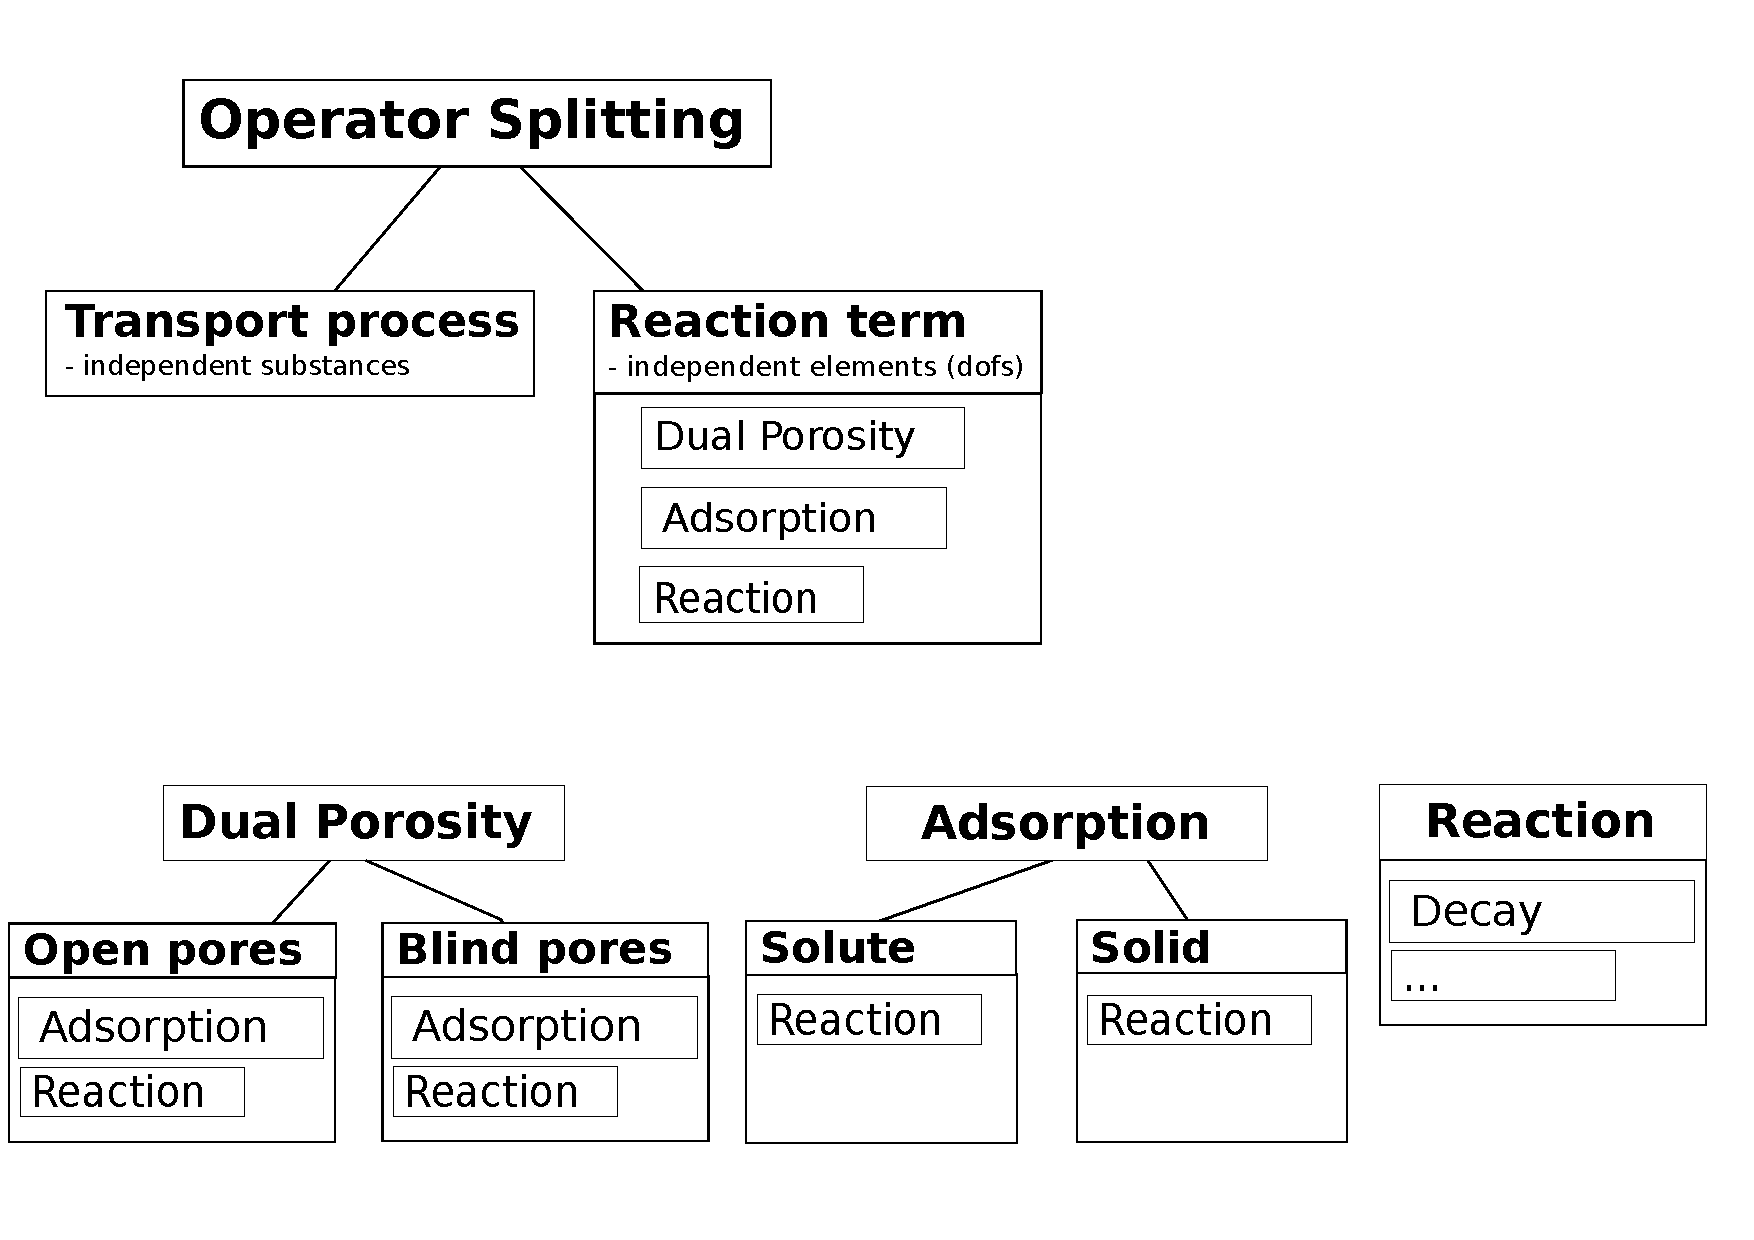
\includegraphics[width=\textwidth]{\fig/reaction_term.pdf}
  \caption{The scheme of the reaction term objects. The lines represents connections between different models. 
  The tables under model name include the possible models which can be connected to the model above.}
  \label{fig:reaction_term}
\end{figure}

The \emph{reaction} model acts only on the specified substances and computes exchange of concentration 
among them. It does not have its own output because it only changes the concentration of substances 
in the specified zone where the reaction takes place.
% See Section \ref{sec:linear_reactions} for thorough description.

The \emph{sorption} model describes the exchange of concentration of the substances between liquid and solid. It can be
followed by another \emph{reaction} that can run in both phases. The concentration in solid is an additional output 
of this model. See Subsection \ref{sec:sorp_math}.


The \emph{dual porosity} model, described in Subsection \ref{sec:dual_porosity}, introduces the so called immobile (or dead-end) pores in the matrix. 
The convection process operates only on the concentration of the substances in the mobile zone (open pores) 
and the exchange of concentrations from/to immobile zone is governed by molecular diffusion. This process can be followed by 
\emph{sorption} model and/or chemical \emph{reaction}, both in mobile and immobile zone. The immobile concentration is an
additional output.


\subsection{Dual Porosity} 
\label{sec:dual_porosity}

Up to now, we have described the transport equation for the single porosity model. The dual porosity model splits the mass into 
two zones -- the mobile zone and the immobile zone. Both occupy the same macroscopic volume, however on the microscopic scale, 
the immobile zone is formed by the dead-end pores, where the liquid is trapped and cannot pass through. The rest of the pore volume 
is occupied by the mobile zone. Since the liquid in the immobile pores is immobile, the exchange of the substance is only due 
to molecular diffusion. We consider simple nonequilibrium linear model:
\begin{subequations}
\label{eq:odes_dual_por}
\begin{align}
    \vartheta_m \partial_t c_m &= D_{dp} ( c_i - c_m), \label{eqn:dual_porosity_ode1}\\
    \vartheta_i \partial_t c_i &= D_{dp} ( c_m - c_i), \label{eqn:dual_porosity_ode2}
\end{align}
\end{subequations}
where $c_m$ is the concentration in the mobile zone, $c_i$ is the concentration in the immobile zone and
$D_{dp}$ is a \hyperA{DualPorosity-Data::diffusion-rate-immobile}{diffusion rate} between the zones.
$\vartheta_i$~denotes \hyperA{DualPorosity-Data::porosity-immobile}{porosity of the immobile zone} and 
$\vartheta_m = \vartheta$ the \hyperA{Solute-Advection-FV-Data::porosity}{mobile porosity} from 
transport equation \eqref{e:ADE}. One can also set non-zero \hyperA{DualPorosity-Data::init-conc-immobile}{initial 
concentration in the immobile zone} $c_i(0)$.

To solve the system of first order differential equation, we use analytic solution or Euler's method,
which are switched according to a given error tolerance. See subsection \ref{sec:num_dual_porosity} 
in numerical methods.
 

\subsection{Equilibrial Sorption}
\label{sec:sorp_math}

The simulation of an equilibrium sorption is based on the solution of two algebraic equations, namely the mass balance (in unit volume)
\begin{equation}
\label{eq:mass_balance_sorption}
\th \varrho_l c_l + (1-\th) \varrho_s c_s = c_T = const.
\end{equation}
and an empirical sorption law
\begin{equation}
\label{eq:relation_cs_cl}
c_s = f(c_l),
\end{equation}
given in terms of the so-called isotherm function $f$.  In these equations we use following notation. 
The concentration in the solid phase, $c_s = \frac{m_{sorbed}}{m_s}$ \units{}{}{} is the adsorbed mass of the substance
per the unit mass of the solid adsorbent in a reference volume. The concentration
in the solid can be selected for \Alink{IT::Sorption-OutputFields}{output}.
The concentration in the liquid phase, $c_l = \frac{m}{m_l}$ \units{}{}{} is the mass of dissolved substance
per the unit mass of the liquid. The relation between $c_l$ and the concentration $c$ from 
       the transport equation \eqref{e:ADE} is $c = c_l \varrho_l$.
 Finally, $\theta$ is the porosity, $\varrho_s$ is the \hyperA{Sorption-Data::rock-density}{solid density} i.e. density of a compact rock with zero porosity,
 and $\varrho_l$ is the \hyperA{Sorption::solvent-density}{liquid density}, i.e. density of the solvent.


The form of the isotherm $f$ is determined by the parameter \hyperA{Sorption-Data::sorption-type}{sorption type}:
\begin{center}
\def\arraystretch{2}
\begin{tabular}{|c|c|p{8cm}|}
\hline
\texttt{sorption\_type} & $f(c_l)$ & \\\hline
``$none$'' & $0$ & The sorption model returns zero concentration in solid.\\\hline
``$linear$'' & $k_l\varrho_l c_l$ &\\\hline
``$freundlich$'' & $k_F \varrho_l c_l^{\alpha}$ &\\\hline
``$langmuir$'' & $k_L \varrho_l \frac{\alpha c_l}{1 + \alpha c_l}$ &
       Langmuir isotherm has been derived from thermodynamic laws. The number $k_L\varrho_l$ denotes the maximal amount 
       of sorbing specie which can be kept in an unit volume of a bulk matrix. Coefficient $\alpha$ is 
       a fraction of sorption and desorption rate constant $\alpha = \frac{k_a}{k_d}$.\\\hline
\end{tabular}
\end{center}
Main parameter of these isotherms is the \hyperA{Sorption-Data::distribution-coefficient}{distribution coefficient} $k_i, i\in\{ l,F,L\}$ \units{-1}{3}{}.
Nonlinear isotherms have an \hyperA{Sorption-Data::isotherm-other}{additional parameter} $\alpha$ \units{}{}{}.
Note that older versions of Flow123d prior to 2.0.0 used a different coefficient $k_i$ denoted \texttt{isotherm\_mult} with the unit [mol$\,\mathrm{kg}^{-1}$].
The conversion rule between the old and new distribution coefficient is
\[ k_i^{new} = \frac{M_s}{\varrho_l} k_i^{old}, \]
where $M_s$ stands for the \hyperA{Substance::molar-mass}{molar mass} of a substance.

Concept of the general distribution coefficient is throughly discussed e.g. in \cite{ORIA1999}. Key assumptions about $k$ are:
\begin{itemize}
 \item Density $\rho_l$ in isotherm expressions is technically the density of the solvent used during measurement of $k$, 
 which could be different then the density of the solvent used in calculation.
 E.g. slight changes in the density of water according to variations in chemical composition and isotopes. But usually the difference is negligible. 
 \item Concentrations in both liquid and solid phase are very small. In particular the number of unoccupied adsorption sites 
 dominates the number of occupied sites. 
 \item All adsorption sites are equivalent.
 \item Sorption is understood in general manner including all linear processes that are able to store the substance.
 \item System is considered in thermodynamic equilibrium.
 \item Single distribution coefficient $K$ is specific for combination adsorbent, solvent, substance.
\end{itemize}


Non-zero \hyperA{Sorption-Data::init-conc-solid}{initial concentration} in the solid phase $c_s(0)$ can be set in the input record. 
Now, further denoting \[ \mu_l = \varrho_l \th, \quad \mu_s = \varrho_s\cdot(1-\th), \]
and using \eqref{eq:relation_cs_cl}, the mass balance \eqref{eq:mass_balance_sorption} reduces to the equation
\begin{equation}
 c_T = \mu_l c_l + \mu_s f(c_l),
 \label{eq:nonlin_sorption}
\end{equation}
which can be either solved iteratively or using interpolation. See subsection \ref{sec:num_sorp_math} 
in numerical methods for details.

The units of $c_l$, $c_s$ and $k_i$ can vary in literature. For an example of conversion rules 
in the case of Freundlich isotherm we refer to Bowman~\cite{bowman_conversion_1982}.

% \paragraph{Units conversion.} Let us have $c$ \units{1}{-3}{}, the mass concentration in liquid, and $s$~[kg\,$\mathrm{kg}^{-1}$], 
% the fraction of the amount of the solute adsorbed and the amount of the adsorbent in solid. 
% The unit of $K$ follows from the dimensional analysis of $s=Kc^{\alpha}$:
% \[[K] = \frac{\rm{kg}^{1-\alpha}\rm{m}^{3\alpha}}{\rm{kg}},\]
% which we want to convert to $k_F$ [mol\,$\mathrm{kg}^{-1}$] in the formula $c_s=k_Fc_l^\alpha$.
% 
% The first step is a conversion of the mass of the solute to moles by dividing it by the
% molar mass $M_s$. We then have the formula 
% \begin{eqnarray}
% s&=&Kc^{\alpha} \nonumber \\
% \frac{s}{M_s} &=& K'\left(\frac{c}{M_s}\right)^\alpha, \label{eqn:sorp_molar_conc}\\
% s &=& K'M_s^{1-\alpha}c^\alpha, \nonumber 
% \end{eqnarray}
% where $s=c_sM_s$ and $K'=KM_s^{\alpha-1}$ [$\rm{mol}^{1-\alpha}\rm{kg}^{-1}\rm{m}^{3\alpha}$] is a new constant,
% distributing the molar concentration in liquid to the ratio of the molar mass and the amount of sorbent in solid.
% 
% The second step is introducing $c_l = \frac{c}{\varrho_l}$ into the formula \eqref{eqn:sorp_molar_conc}
% \begin{equation}
% c_s = K'\left(\frac{c_l \rho_l }{M_s}\right)^\alpha
% = K' M_s^{-\alpha}\rho_l^{\alpha}c_l^\alpha 
% = \left( K M_s^{-1}\rho_l^{\alpha} \right) c_l^\alpha,
% \end{equation}
% where we can denote 
% \begin{equation}
% k_F=K M_s^{-1}\rho_l^{\alpha},
% \end{equation} 
% which is the constant we are looking for. This can be also translated to the case of the linear isotherm, where
% $\alpha=1$ and $[K] = \rm{kg}^{-1}\rm{m}^{3}$, and we get the conversion rule
% \begin{equation}
% k_l=K M_s^{-1}\rho_l.
% \end{equation} 
% The conversion of different prefixes of units are left on the user. One should be careful using the 
% Freundlich isotherm, though, where the exponent $\alpha$ must not be forgotten.


\subsection{Sorption in Dual Porosity Model} 
\label{subsec:sorp_dual_por}
There are two parameters $\mu_l$ and $\mu_s$, scale of aqueous concentration and scale of sorbed concentration, respectively.  
There is a difference in computation of these in the dual porosity model because both work on different concentrations
and different zones.

Let $c_{ml}$ and $c_{ms}$ be concentration in liquid and in solid in the mobile zone, 
$c_{il}$ and $c_{is}$ be concentration in liquid and in solid in the immobile zone,
$\vartheta_m$ and $\vartheta_i$ be the mobile and the immobile porosity,
and $\varphi$ be the sorbing surface.

The sorbing surface in the mobile zone is given by
\begin{equation}
  \varphi = \frac{\vartheta_m}{\vartheta_m + \vartheta_i}, 
\end{equation}

while in the immobile zone it becomes
\[ 1 - \varphi = 1-\frac{\vartheta_m}{\vartheta_m + \vartheta_i} = \frac{\vartheta_i}{\vartheta_m + \vartheta_i}. \]

Remind the mass balance equation \eqref{eq:nonlin_sorption}.
In the dual porosity model, the scaling parameters $\mu_l$, $\mu_s$ are slightly different.
In particular, the mass balance in the mobile zone reads:
\begin{eqnarray}
 \begin{array}{l}
  c_T = \mu_l\cdot c_{ml} + \mu_s\cdot c_{ms},\\
  \mu_l = \varrho_l \cdot \vartheta_m, \\
  \mu_s = \varrho_s\cdot(1-\vartheta_m - \vartheta_i)\varphi,
 \end{array}
 \label{eq:scale_params_m}
\end{eqnarray}
while in the immobile zone it has the form:
\begin{eqnarray}
 \begin{array}{l}
  c_T = \mu_l\cdot c_{il} + \mu_s\cdot c_{is},\\
  \mu_l = \varrho_l \cdot \vartheta_i, \\
  \mu_s = \varrho_s\cdot(1-\vartheta_m - \vartheta_i)(1 - \varphi).
 \end{array}
 \label{eq:scale_params_i}
\end{eqnarray}
